\documentclass[convert={density=300,size=1080x800,outext=.png}]{standalone}
\usepackage{xcolor}
\usepackage{graphics, graphicx}
\usepackage{tikz, tkz-graph}
\usepackage{pgf, pgfplots}
\usepackage{graphviz, tkz-berge}
\usepackage{graphics, graphicx}
\usepackage{pstricks, pst-node, pst-tree}

\usetikzlibrary{arrows, petri, topaths}
\usetikzlibrary{shapes}
\usetikzlibrary{arrows.meta}
\usetikzlibrary{positioning,automata}



\begin{document}
		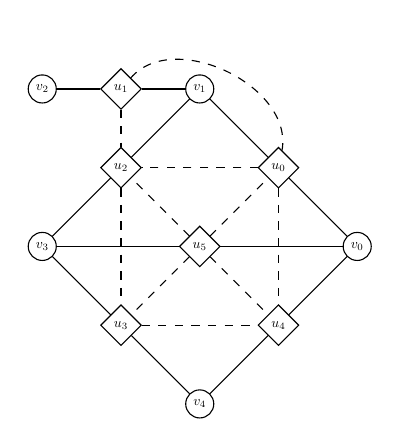
\begin{tikzpicture}[round/.style={circle, draw=black, thin, minimum size=.5mm}, transform shape, scale=0.5]
			\node[round] (a) at (8,4){$v_{0}$};
			\node[round] (b) at (4,8){$v_{1}$};
			\node[round] (c) at (0,8){$v_{2}$};
			\node[round] (d) at (0,4){$v_{3}$};
			\node[round] (e) at (4,0){$v_{4}$};
			\node[draw, diamond] (f) at (6,6){$u_{0}$};
			\node[draw, diamond] (g) at (2,8){$u_{1}$};
			\node[draw, diamond] (h) at (2,6){$u_{2}$};
			\node[draw, diamond] (i) at (2,2){$u_{3}$};
			\node[draw, diamond] (j) at (6,2){$u_{4}$};
			\node[draw, diamond] (k) at (4,4){$u_{5}$};
			\draw (a) edge (f);
			\draw (a) edge (j);
			\draw (a) edge (k);
			\draw (f) edge (b);
			\draw (j) edge (e);
			\draw (k) edge (d);
			\draw (b) edge (g);
			\draw (g) edge (c);
			\draw (b) edge (h);
			\draw (h) edge (d);
			\draw (d) edge (i);
			\draw (i) edge (e);
			
			\draw (f) edge[dashed] (h);
			\draw (k) edge[dashed] (f);
			\draw (k) edge[dashed] (j);
			\draw (k) edge[dashed] (i);
			\draw (k) edge[dashed] (h);
			\draw (f) edge[dashed] (h);
			\draw (i) edge[dashed] (j);
			\draw (g) edge[dashed] (h);
			\draw (f) edge[dashed] (j);
			\draw (h) edge[dashed] (i);
			\draw (g) edge[dashed, bend left=75] (f);
			
		\end{tikzpicture}

\end{document}